\documentclass{beamer}
\usepackage{HECbeamer}
% \usepackage{pgfpages}
% \pgfpagesuselayout{4 on 1}[letterpaper, landscape, border shrink=5mm]
\title[\color{white}{MATH 60604A \S~6d - Random intercept model}]{\texorpdfstring{MATH 60604A \\Statistical modelling \\ \S~6d  - Random intercept model}{MATH 60604A \\Statistical modelling \\ \S~6d - Random intercept model}}
\author{}
\institute{HEC Montréal\\
Department of Decision Sciences}
\date{} 

\begin{document}
\frame{\titlepage}




\begin{frame}[fragile]
\frametitle{Random intercept linear model}
\bi
\item The simplest random effects model is one with only a group-specific random intercept. 
\item The equation of the linear mixed model is
\begin{align*}
Y_{ij}=\beta_0 + b_i + \beta_1 \mathrm{X}_{ij1}+\cdots+\beta_p\mathrm{X}_{ijp} + \varepsilon_{ij}, \qquad  \bs{\varepsilon}_{i} \sim \mathsf{No}(\bs{0}, \mathbf{R}_i)
\end{align*}
for $i=1, \ldots, m$ and $j=1, \ldots, n_i$ and where $Y_{ij}$ is observation $j$ from group $i$.
\item The intercept specific to group $i$ is $\beta_0+b_i$. It consists of
\bi

\item A \textbf{common effect over all groups}, $\beta_0$;
\item A \textbf{group-specific effect}, $b_i$.
\ei 
\ei
\end{frame}

\begin{frame}[fragile]
\frametitle{Graphical illustration}
Consider a random intercept model for the \texttt{revenge} data, with $\mathsf{AR}(1)$ errors and \texttt{t} as fixed effect.
\begin{center}
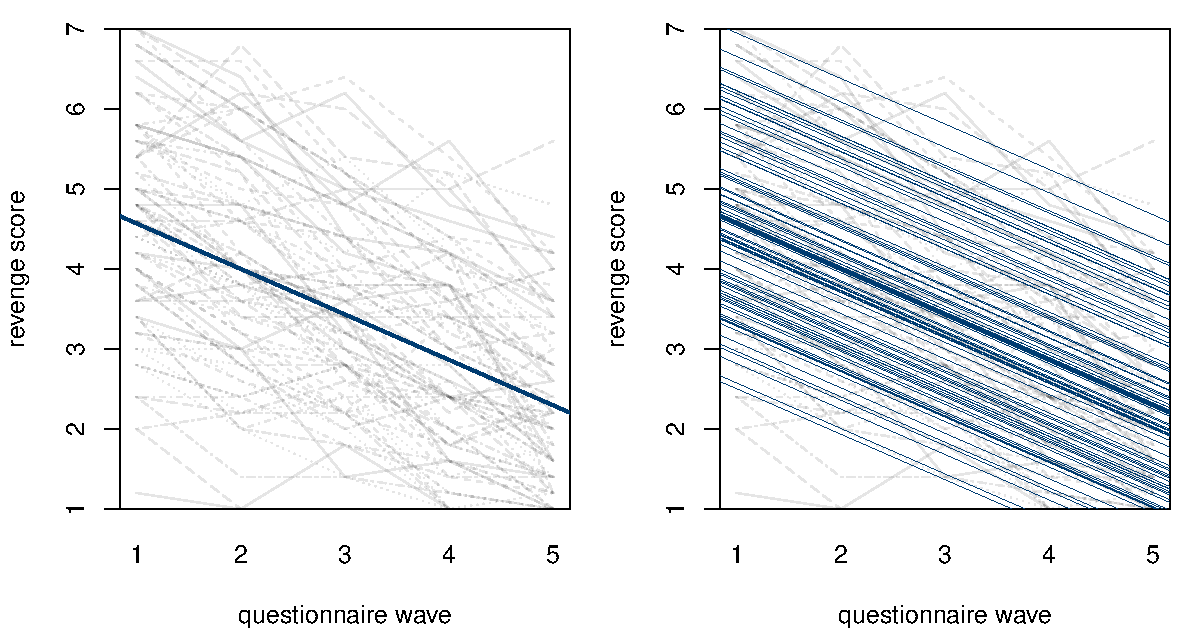
\includegraphics[width = 0.8\linewidth]{img/c6/07-mixed-randomintercept}
\end{center}
{\footnotesize 
Model without (left) and with random intercept for \texttt{id} (right).

}
\end{frame}

\begin{frame}[fragile]
\frametitle{Assumptions of the random intercept model}
The model equation is
\begin{align*}
Y_{ij}=(\beta_0+b_i)+ \beta_1 \mathrm{X}_{ij1}+\beta_2\mathrm{X}_{ij2}+\cdots+\beta_p\mathrm{X}_{ijp} + \varepsilon_{ij}
\end{align*}
\bi
\item The random effects $b_1, \ldots, b_m$ are assumed to be \alert{independent} from the $\varepsilon$ terms and the explanatory variables).
\item We assume for the time being
\bi \item $b_{i\phantom{j}}\simiid \mathsf{No}(0, \sigma^2_b)$ $(i=1, \ldots, m)$.
\item $\varepsilon_{ij}\simiid \mathsf{No}(0, \sigma^2)$  $(i=1, \ldots, m; j = 1, \ldots, n_i)$.
\ei
% \item The $\varepsilon_{ij}$ terms could be correlated within group $i$, but they are assumed independent for the time being.
\ei
\end{frame}



\begin{frame}[fragile]
\frametitle{Random effects models: covariance}

Since it's random, the term $b_i$ introduces a \alert{within-group correlation in the model}. Because $\eps_{ij}$ is independent of $b_i$ for all $i, j$, the (conditional) variance of an observation is
\begin{align*}
\Va{Y_{ij}\mid \mathbf{X}_i}&=\Va{b_i}+\Va{\varepsilon_{ij}}=\sigma^2_b + \sigma^2_{\vphantom{b}}
\end{align*}
The covariance between two individuals in the same group is
\begin{align*}
\Co{Y_{ij}, Y_{ik}\mid \mathbf{X}_i}=\sigma^2_b, \qquad j\neq k.
\end{align*}
Consequently, the correlation between two individuals in the same group is
\begin{align*}
\Cor{Y_{ij}, Y_{ik}\mid \mathbf{X}_i}=\frac{\sigma^2_b}{\sigma^2_{\vphantom{b}}+\sigma^2_b}, \qquad  j\neq k.
\end{align*}
This quantity is often called the \alert{intra-class correlation}.

\end{frame}
\begin{frame}{Mathematical aside}
Both  $\beta_j$ and explanatories are assumed non-random, thus
 \begin{align*}
  \Co{Y_{ij}, Y_{ik} \mid \mathbf{X}_i} &= \mathsf{Co}\left(\beta_0 +b_i + \beta_1\mathrm{X}_{ij1}+\cdots + \eps_{ij},\right.\\
  & \quad \qquad \left.\beta_0 +b_i + \beta_1\mathrm{X}_{ik1}+\cdots + \eps_{ik} \mid \mathbf{X}_i\right)
  \\&= \Co{b_i+ \eps_{ij}, b_i + \eps_{ik}}
  \\&= \Va{b_i} + \Co{\eps_{ij}, \eps_{ik}} \\&= \sigma^2_b +\sigma^2\I{j=k}.
\end{align*}
where the last step follows from independence of $b_i$ and $\eps$'s and because $\Co{Y_{ij},Y_{ij}}=\Va{Y_{ij}}$.

\end{frame}
\begin{frame}{Unconditional variance of $\bs{Y}$}


Alternatively,
\begin{align*}
   \Va{\bs{Y}_i \mid \mathbf{X}_i} &= \Va{b_i \bs{1}_{n_i}} + \Va{\bs{\eps}_i}
%    \\&=
%    \begin{matrix} b_i \\ \vdots \\ b_i 
%    \end{matrix}
%    } + \Va{\begin{matrix}\eps_{i1} \\ \vdots \\ \eps_{in_i}\end{matrix}}
   \\&= \sigma^2_b \bs{1}_{n_i}\bs{1}_{n_i}^\top + \sigma^2 \mathbf{I}_{n_i}
   \\&= 
   \begin{pmatrix}
 \sigma^2_b &  \sigma^2_b & \cdots & \sigma^2_b \\
  \sigma^2_b &  \sigma^2_b & \cdots & \sigma^2_b \\
 \vdots & \ddots & \ddots & \vdots \\
 \sigma^2_b &  \sigma^2_b & \cdots & \sigma^2_b   
 \end{pmatrix} + \begin{pmatrix}
 \sigma^2 & 0 & \cdots &0\\
 0 & \sigma^2 & \ddots &0\\
 \vdots &\ddots & \ddots & \vdots\\
 0 & 0 & \cdots & \sigma^2
 \end{pmatrix}.
\end{align*}

\end{frame}


\begin{frame}[fragile]
\frametitle{Compound symmetry correlation induced by the random intercept model}

\bi \item 
When the error terms $\bs{\eps}_i$ are independent with $\Va{\bs{\eps}_i}=\sigma^2\mathbf{I}_{n_i}$, introducing a random effect $b_0$ for the intercept implies that the within-group correlation is the same.
\item 
In that particular case, the conditional covariance matrix of $\boldsymbol{Y}_i$ is thus the same as if we considered a linear regression model with no random effect and a compound symmetry model for $\Va{\bs{\eps}_i}$.
\item 
The difference is that now the correlation must be non-negative, since $\sigma^2_b$ is a variance. This limitation is not usually of consequence, because within-group correlations tend to be positive.
\ei
\end{frame}
% \begin{frame}
% \frametitle{Compound symmetry}
% \bi
% \item The difference is that now the correlation must be non-negative, since $\sigma^2_b$ is a variance whereas the correlation for the compound symmetry model was \[-\frac{1}{\max(n_i)+1} \leq \rho \leq 1.\]
% \item This limitation is not usually of consequence, because within-group correlations tend to be positive.
% 
% \ei
% \end{frame}


\begin{frame}[fragile]
\frametitle{Adding a random intercept with the \code{random} command} 
\bi 
\item The command \code{repeated} allows us to specify the covariance structure for the errors in \code{proc mixed}. 
\item If we don't use the \texttt{repeated} command, the errors are assumed to be independent.
\ei
\begin{tcolorbox}[colback=white, colframe=hecblue, title=\SASlang{} code for a random intercept model with independent errors]
\begin{small}
\begin{verbatim}
proc mixed data=statmod.motivation; 
class idunit; 
model motiv = sex yrserv agemanager nunit / solution; 
random intercept / subject=idunit v=1 vcorr=1; 
run;
\end{verbatim}
\end{small}
\end{tcolorbox}
{ \footnotesize   Including a random intercept \alert{induces} a compound symmetry correlation structure.
Therefore, we do not need to specify anything for the covariance structure of the errors.


}
\end{frame}
% 
% \begin{frame}[fragile]
% \frametitle{Remarks on the \SASlang{} code}
% \bi
% \item It's important to note that we have not assumed any structure on the covariance of the errors here --- there is no \texttt{repeated} command in the \SASlang{} code.
% \item As we've already seen, including a random intercept \alert{naturally} induces a compound symmetry correlation structure.
% \item Therefore, we do not need to specify anything for the covariance structure of the errors.
% \ei
% \end{frame}
% 
% \begin{frame}[fragile]
% \frametitle{Model specification}
% \begin{center}
% \includegraphics[scale=0.5]{Figures/long88.pdf}
% \end{center}
% \end{frame}

\begin{frame}[fragile]
\frametitle{Covariance matrix specified by the random intercept model}
\begin{center}
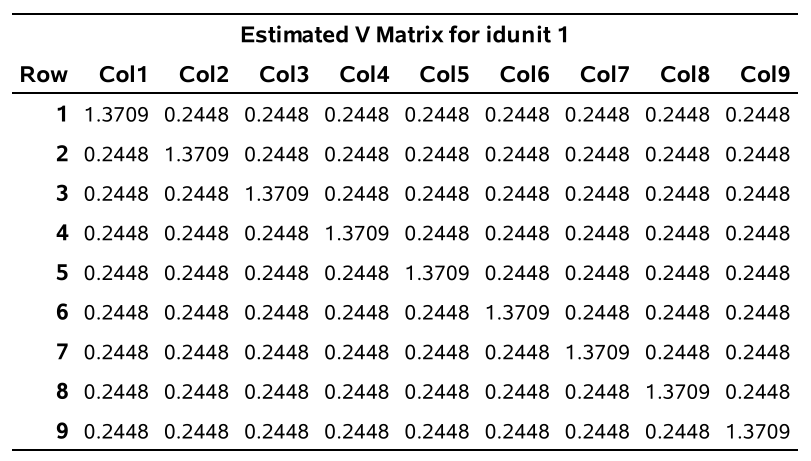
\includegraphics[width = 0.9\linewidth]{img/c6/slides7-e11}

\end{center}
\end{frame}

% \begin{frame}[fragile]
% \frametitle{Correlation matrix for the data}
% \begin{center}
% 
% \end{center}
% \end{frame}

\begin{frame}[fragile]
\frametitle{Covariance parameter estimates}
\begin{center}
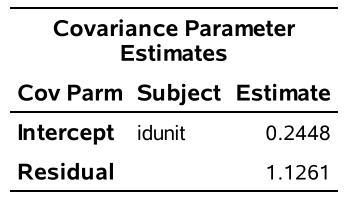
\includegraphics[width = 0.4\linewidth]{img/c6/slides7-e12}
\end{center}
\bi
\item The variance estimate for the random intercept is
$\hat{\sigma}^2_b=0.2448$, whereas the estimate of the variance of the error term is
$\hat{\sigma}^2= 1.1261$.
\item Consequently, the estimate of the within-unit correlation is
\begin{align*}
\hat{\rho}=\frac{\hat{\sigma}^2_b}{\hat{\sigma}^2_b+\sigma^2_{\vphantom{b}}}=0.1785.
\end{align*}
% \item This agrees with the value reported in the correlation matrix for individual 1. 
\item This is exactly the same correlation for the observation than that obtained from compound symmetry covariance model for the errors (command \code{repeated}).
\ei
\end{frame}

\begin{frame}[fragile]
\frametitle{Fixed effect estimates}
\begin{center}
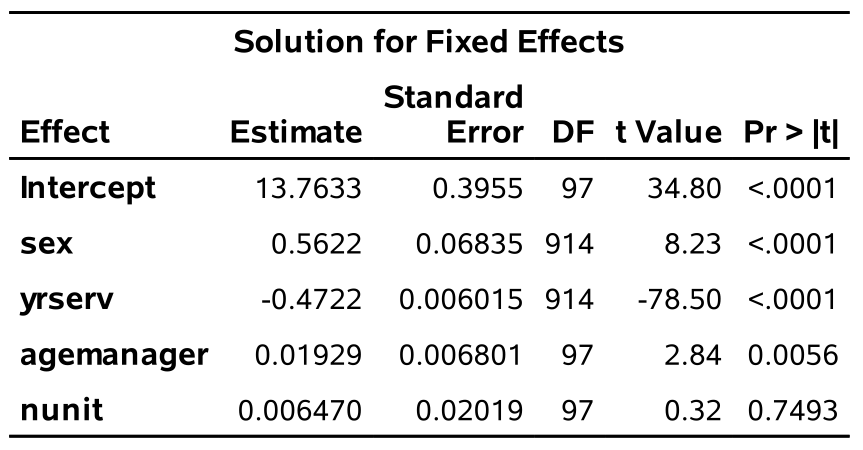
\includegraphics[width = 0.7\linewidth]{img/c6/slides7-e10}
\end{center}
{\footnotesize The effects of the explanatory variables (and their standard errors)
are also the same as for the compound symmetry structure --- both models are equivalent for the response assuming the within-unit correlation is positive. 


}
\end{frame}
% \begin{frame}[fragile]
% \frametitle{Investigation of the usefulness of the random intercept}
% \bi
% \item Testing whether the variance of the random effect $\sigma^2_b=0$ (no random intercept) is a non-standard testing problem \ldots 
% \item The model which includes a random intercept and an $\mathsf{AR}(1)$ covariance structure within-unit for the residuals had a $\mathsf{BIC}$ ($\mathsf{AIC}$) of $694.4$ ($687.2$) compared to $690.5$ ($685.8$) for the model without random effects.
% \item According to the $\mathsf{BIC}$, the best model is the one without a random effect, but with an $\mathsf{AR}(1)$ correlation on the errors. $\mathsf{AIC}$ prefers more complicated models and so includes the random intercept.
% \item It seems that modelling an intercept for each subject is not necessary in this example. The $\mathsf{AR}(1)$ correlation of the errors appears to be sufficient in explaining the correlation in the data.
% \ei
% \end{frame}

\end{document}
